\RequirePackage{plautopatch}
\documentclass[upLaTeX,a4paper]{jsarticle}
\usepackage{listings,jlisting,amsmath,otf,here,empheq}
\usepackage[dvipdfmx]{graphicx}

\lstset{
breaklines = true,
numbers = left,
frame = tbrl,
tabsize = 4,
captionpos = t
}

\title{流体の数値計算プログラムの作成 レポート 修正版2}
\author{B4 津田修一朗}
\date{2021/6/15}

\begin{document}
\maketitle

具体的な手法については前回、前々回のレポートで述べたため、このレポートでは前回レポートからの修正点を中心に議論する。

\section{数値計算の手順,手法}
\subsection{流れ関数と渦度を求めるプログラムの実装}
流れ関数-渦度法により,cavity内の流れを解いた.
今回は基礎方程式の実装を修正した。

また、これまでは収束条件を流れ関数$varPsi$ 渦度$\omega$のイテレーションごとの差がともに0.00001以下になることとしていたものを,0.000001に変更した.
これにより、cavity底付近の逆流渦が大きくなることが確認できたため,前回の条件では十分に収束に至っていなかったことが考えられる.

ただし、収束条件を厳しくした結果,格子点$151 × 151$に設定した時にはプログラムを実行してから30分程度経過しても収束条件を満たさなかった。
そのため,今回は(i)レイノルズ数$Re = 50$, 格子点$51\times 51$, (ii)レイノルズ数$Re = 200$, 格子点$101\times 101$
でシミュレーションを行った.

\subsection{速度ベクトル図の描画}
cavity底面付近の逆流渦の挙動を確認する為に、各格子点における速度ベクトルをその大きさで割り,
流れの方向が分かりやすくなるようにした図を追加した.

\subsection{流線図の描画}
流線は流れ関数$\varPsi = const$で表されることを用いて,流れ関数と渦度を求めるプログラムにより求めた流れ関数を用いて流線図を描画した.

\subsection{等圧線図の描画}
前回までは圧力のポアソン方程式を用いた差分方程式により圧力場を求めていたが,確からしい結果が得られなかったため,\cite{2}で紹介された方法を用いた.
無次元化されたNavier-Stokes方程式は,

\begin{equation}
  \begin{split}
    \frac{\partial u}{\partial t}
  \end{split}
\end{equation}

\section{数値計算の結果}
\subsection{速度ベクトル図}
図1,2,3に今回得られた速度ベクトル図を示す.これらの図より,$(0,1),(1,1)$間を結ぶ線分に相当する移動壁面付近で比較的速い流れが生じ,cavity内に1つの渦ができていることが確認できる.
また,レイノルズ数$Re$が大きくなるにつれて、渦の中心が点(1, 1)に近づくことが確認できる.
さらに,レイノルズ数$Re=500$のときには$y=0$付近で流体の速さがおおよそ0であることがわかった.
\begin{figure}[H]
  \centering
  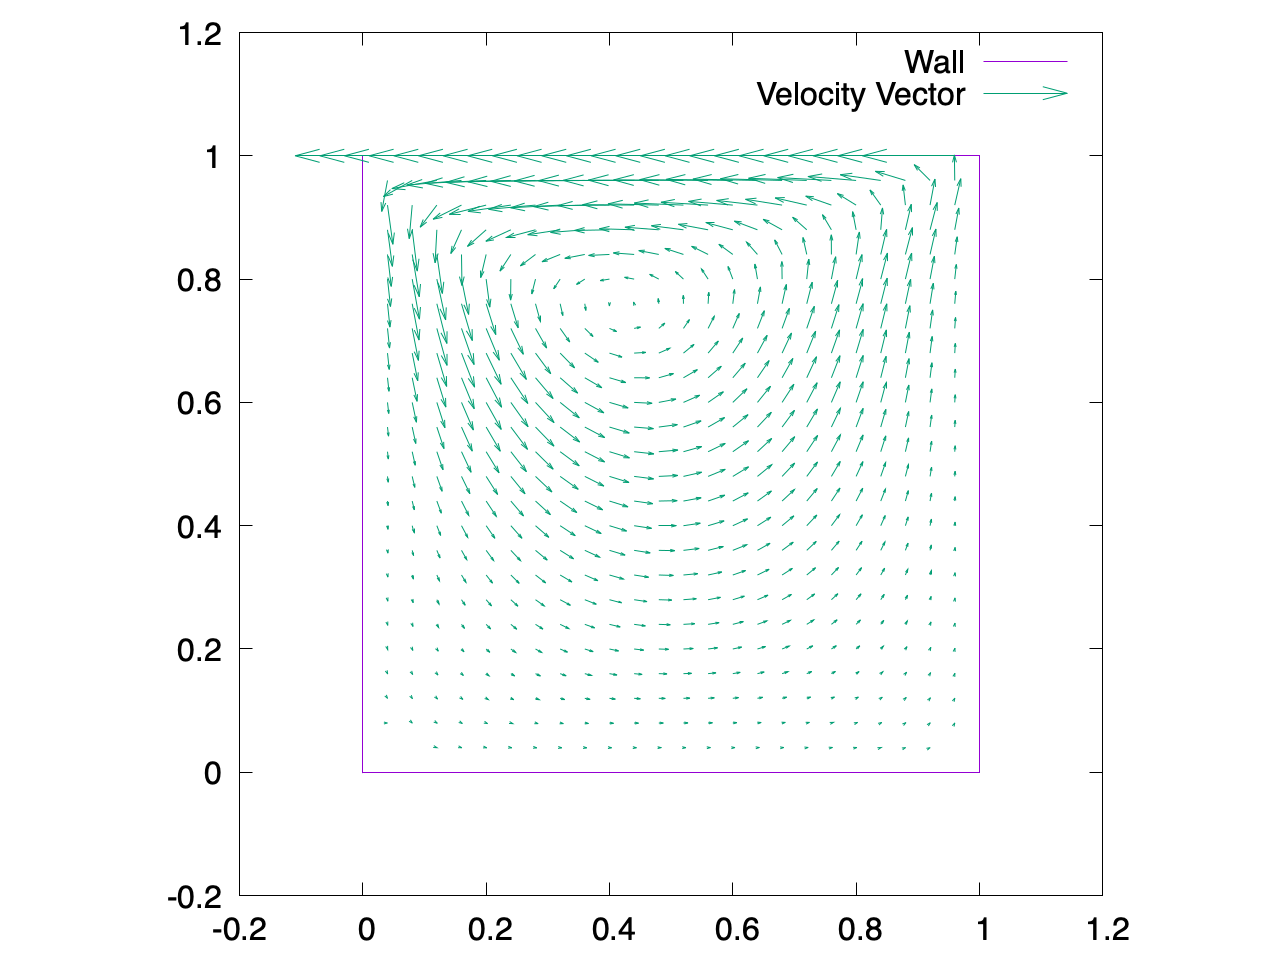
\includegraphics[height=9.5cm]{outputs/img/velocity_vector_re50.png}
  \caption{速度ベクトル図(i)}
  \label{fig:velocity_vector_re50}
\end{figure}
\begin{figure}[H]
  \centering
  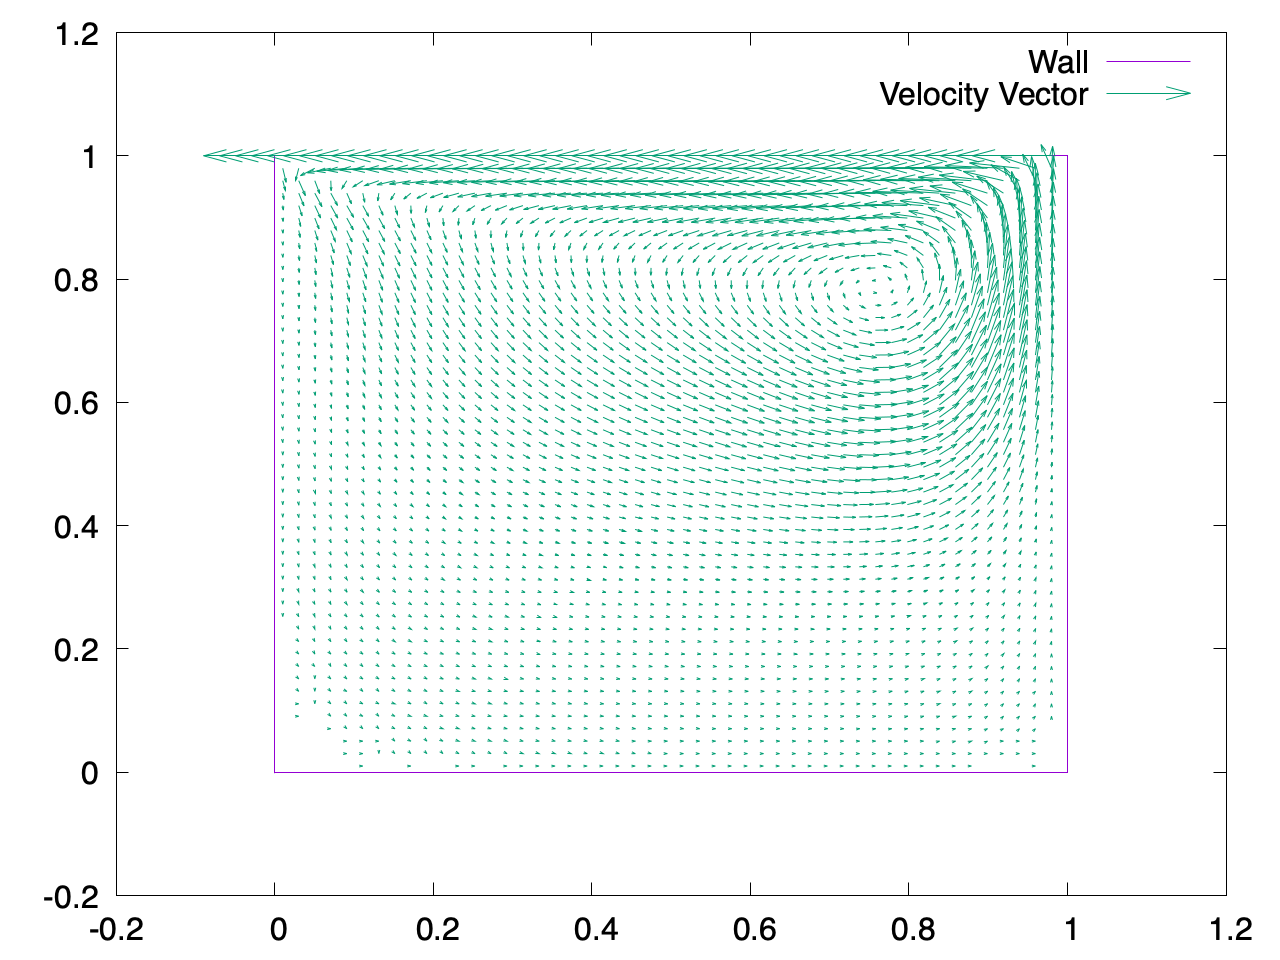
\includegraphics[height=9.5cm]{outputs/img/velocity_vector_re200.png}
  \caption{速度ベクトル図(ii)}
  \label{fig:velocity_vector_re200}
\end{figure}
\begin{figure}[H]
  \centering
  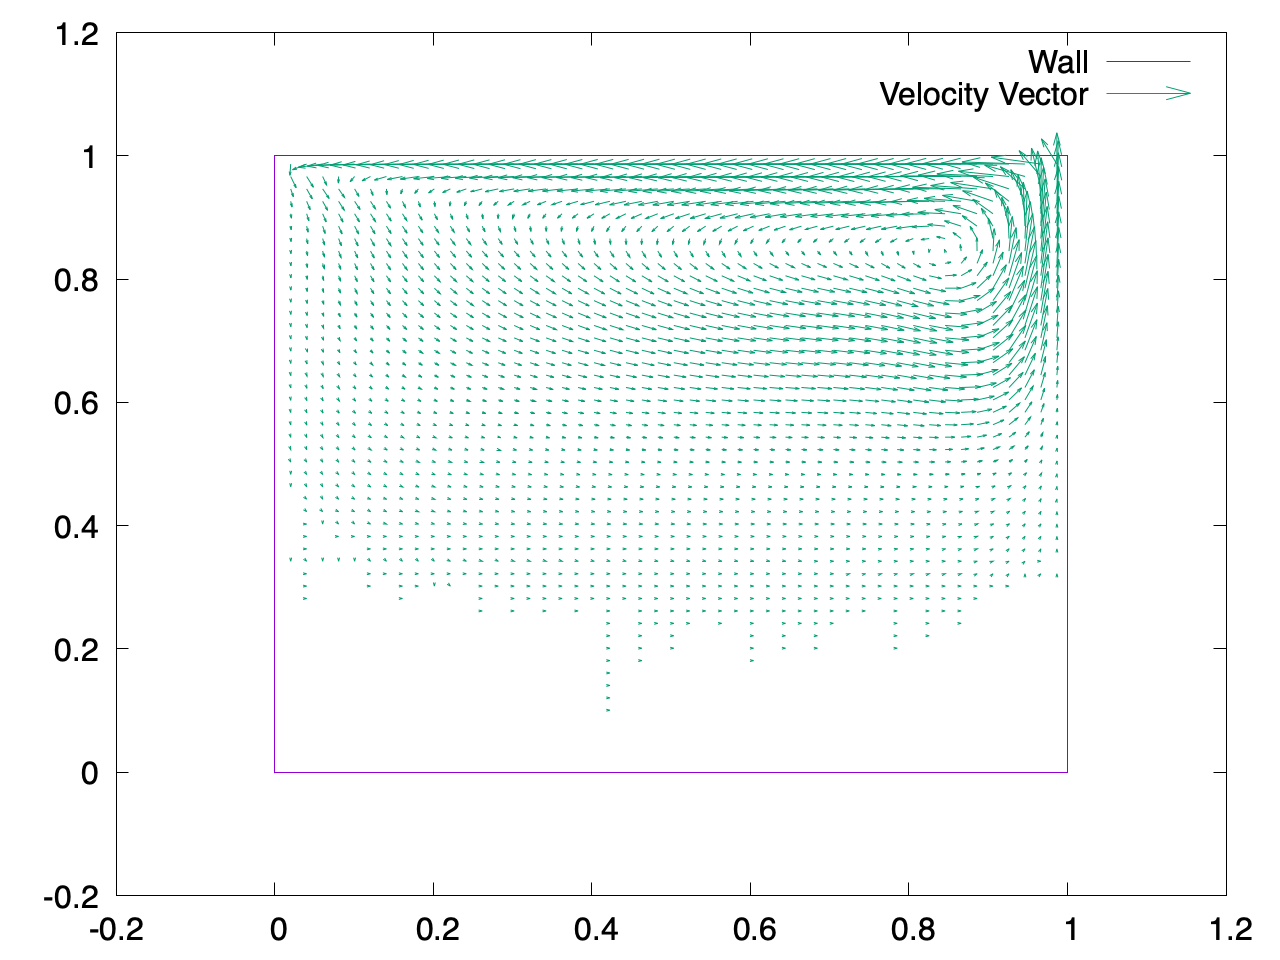
\includegraphics[height=9.5cm]{outputs/img/velocity_vector_re500.png}
  \caption{速度ベクトル図(iii)}
  \label{fig:velocity_vector_re500}
\end{figure}


\subsection{流線図}

図4,5,6に今回得られた流線図を示す.
中間報告においては, gnuplotの格子状データを生成するdgrid3d機能を用いていたため,比較的離れた格子点の情報が入ってしまっていた.
しかし,その後データを格納しているcsvファイルの形式を修正し,dgrid3dを使わず,数値解析によって得られた値をそのまま格子状データとして描画する方法を用いたので,最近接点のみの情報で表現できた.

\begin{figure}[H]
  \centering
  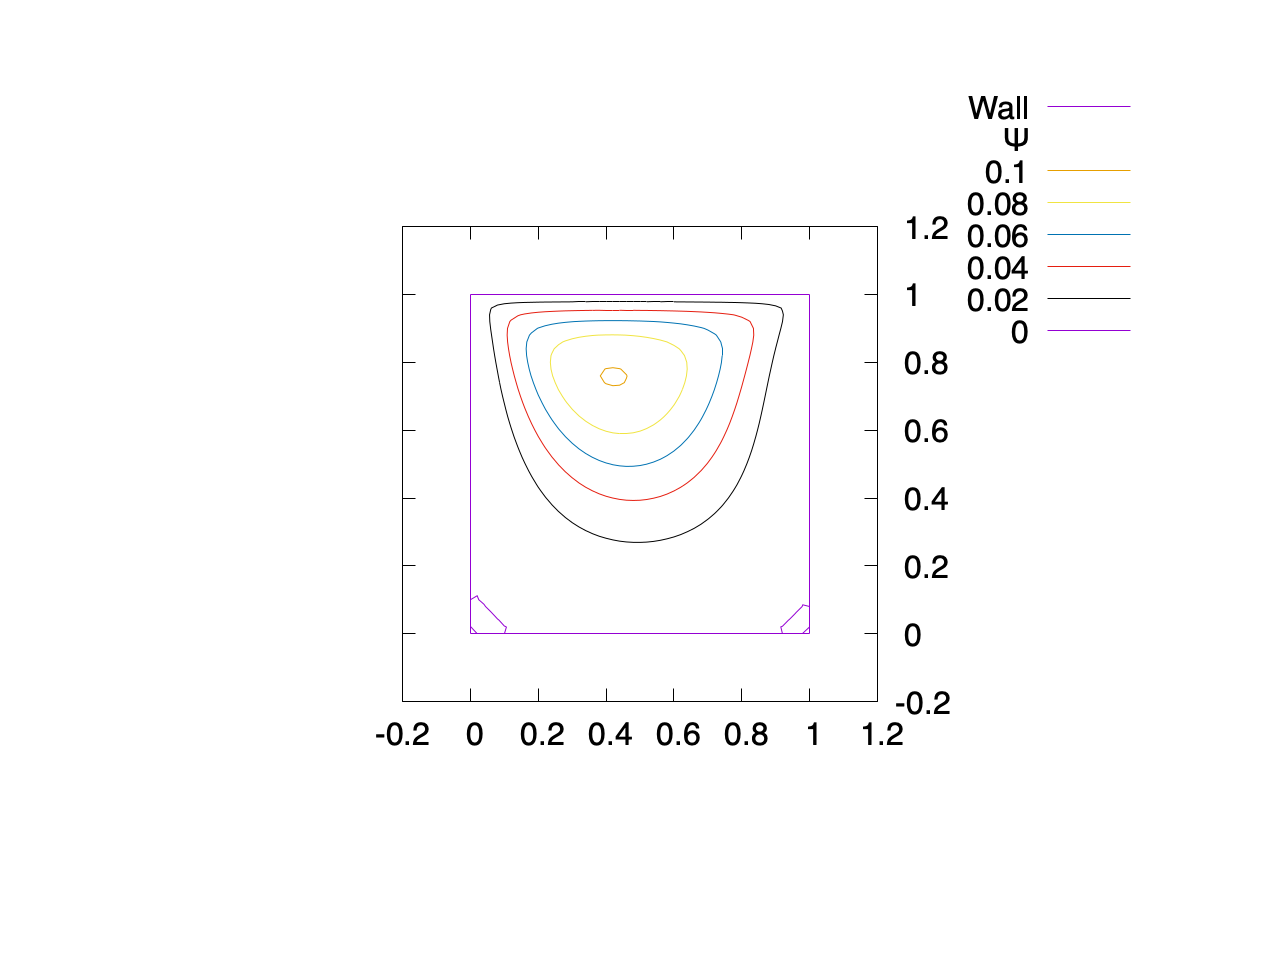
\includegraphics[height=9.5cm]{outputs/img/stream_line_re50.png}
  \caption{流線図(i)}
  \label{fig:velocity_vector_re50}
\end{figure}
\begin{figure}[H]
  \centering
  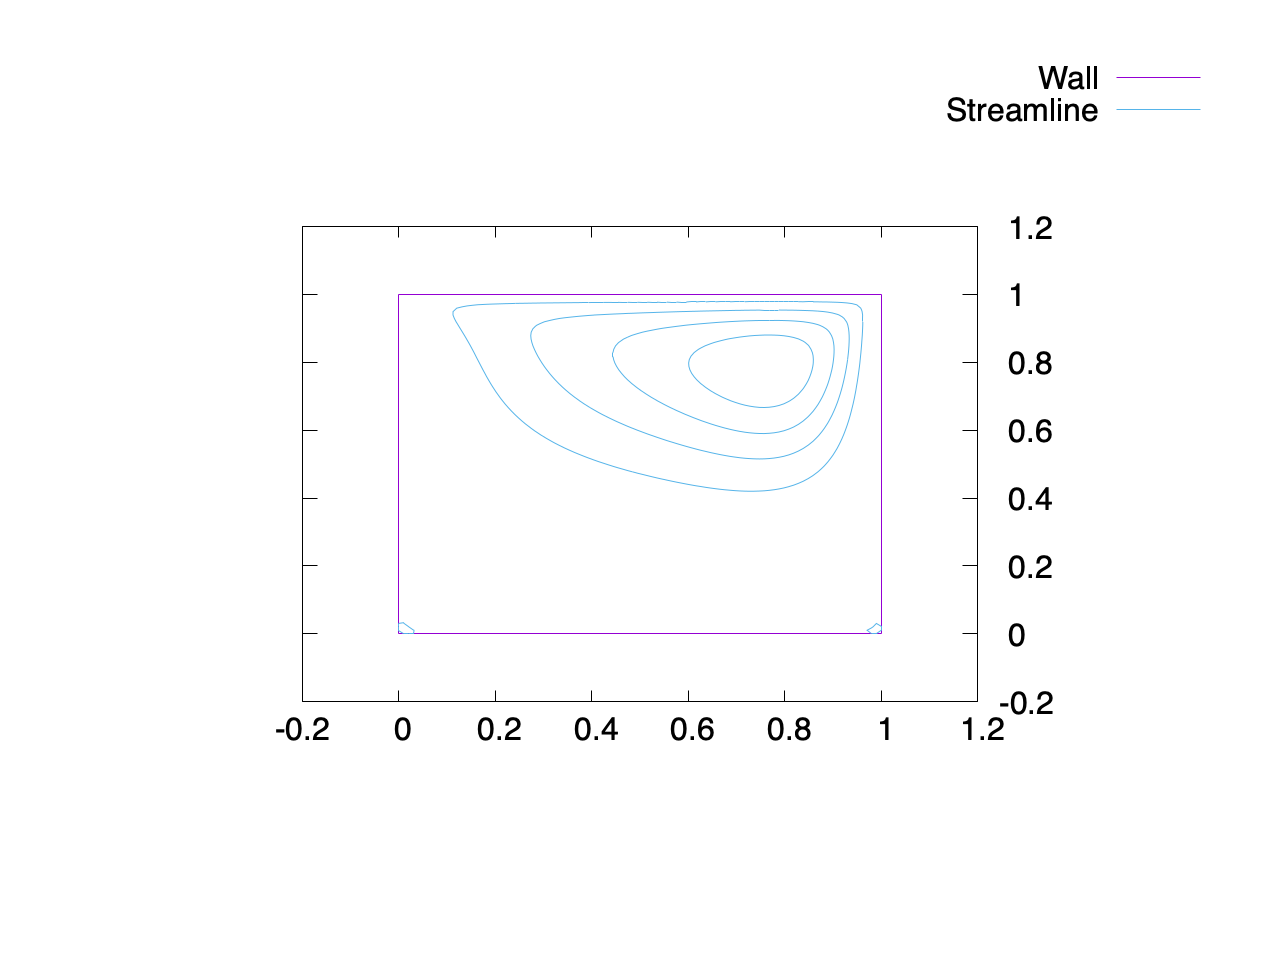
\includegraphics[height=9.5cm]{outputs/img/stream_line_re200.png}
  \caption{流線図(ii)}
  \label{fig:velocity_vector_re200}
\end{figure}
\begin{figure}[H]
  \centering
  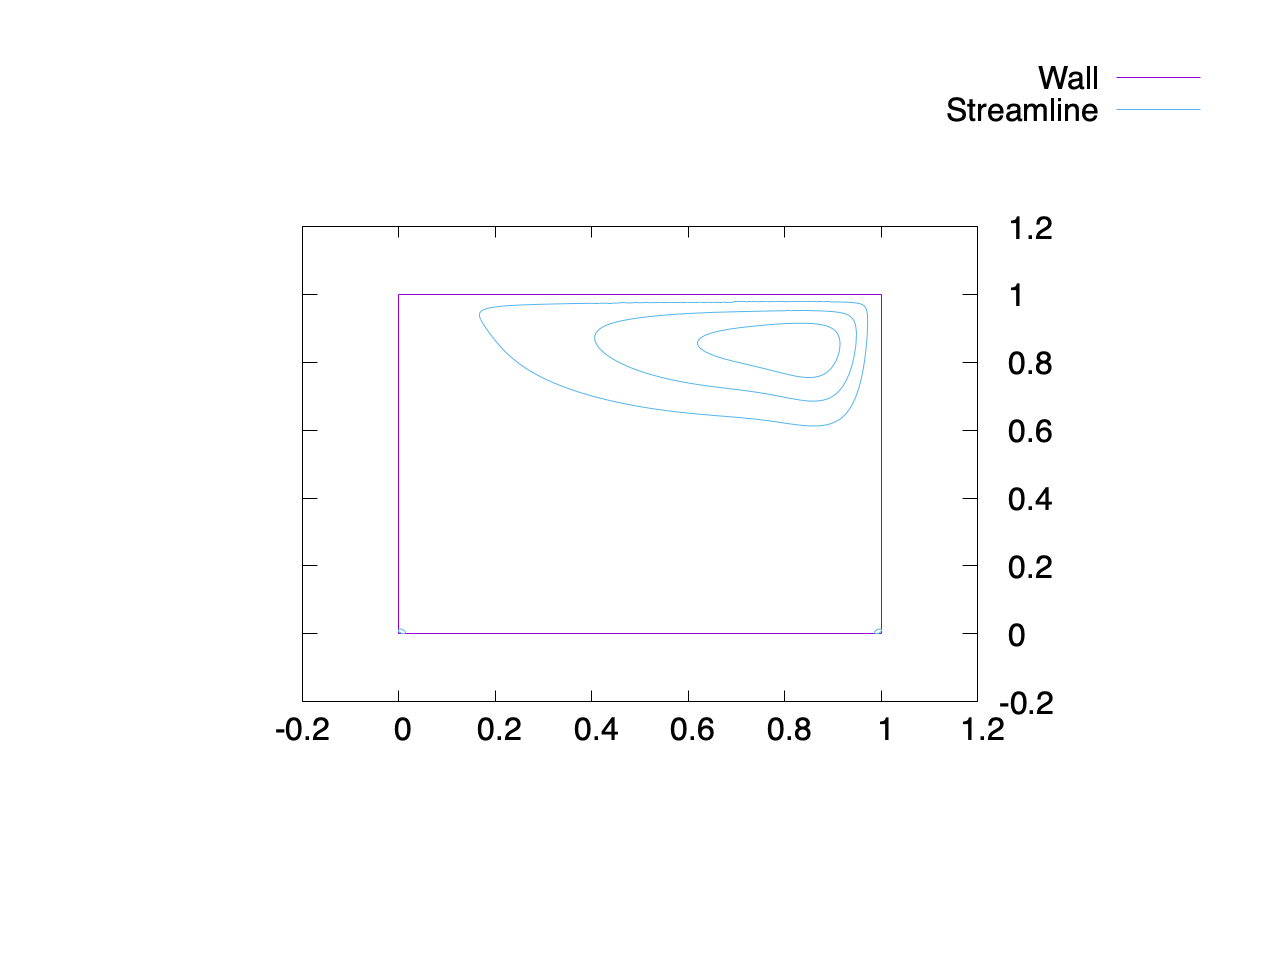
\includegraphics[height=9.5cm]{outputs/img/stream_line_re500.png}
  \caption{流線図(iii)}
  \label{fig:velocity_vector_re500}
\end{figure}


\subsection{等圧線図}
図7,8,9に今回得られた等圧線図を示す.
$(0,0),(1,0)$を結ぶ線分付近で圧力が高く,点(0,1),(1,1)付近で圧力が低い結果となった.
\begin{figure}[H]
  \centering
  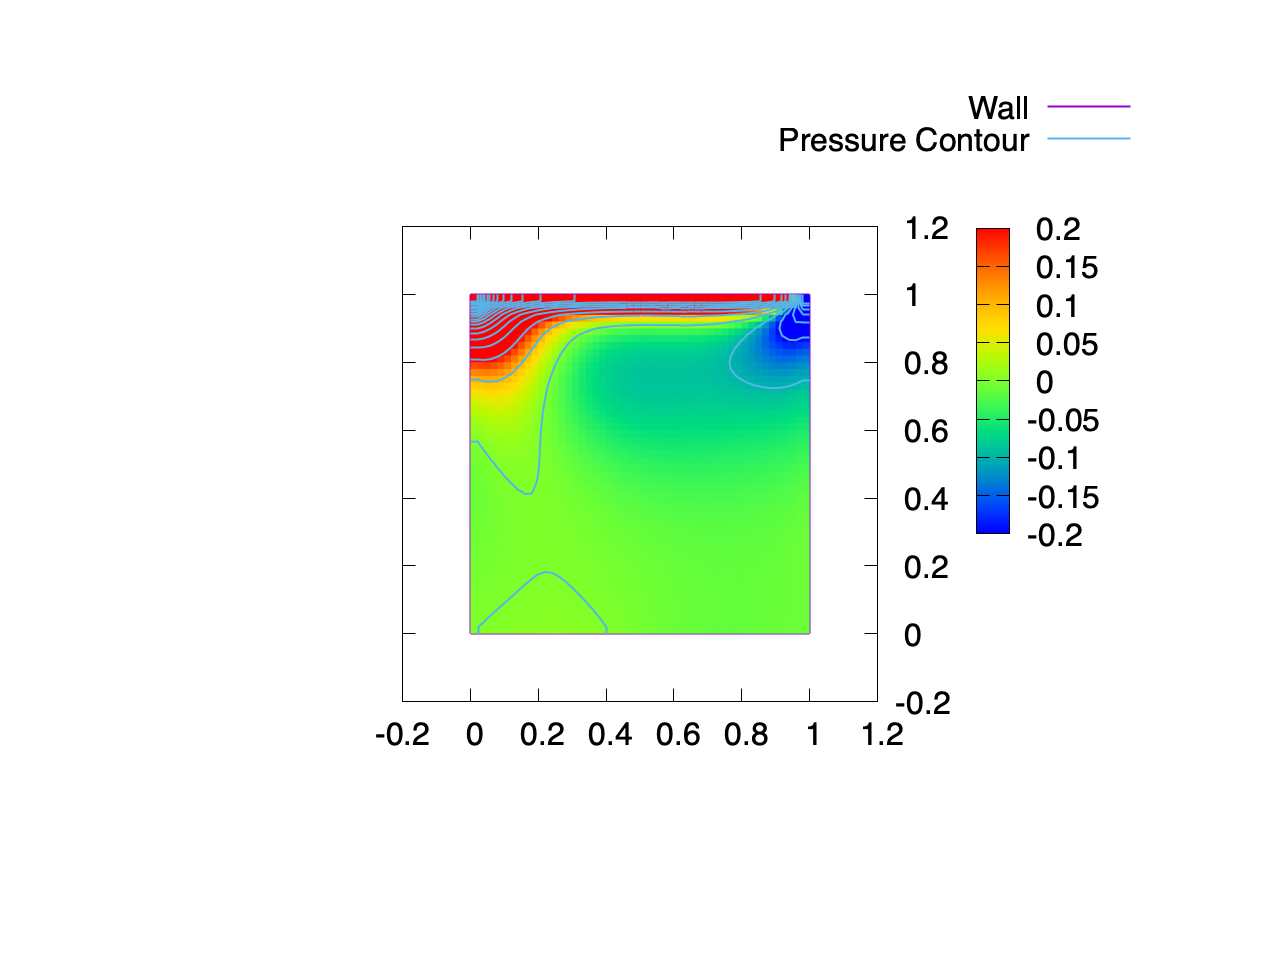
\includegraphics[height=9.5cm]{outputs/img/p_re50.png}
  \caption{等圧線図(i)}
  \label{fig:p_re50}
\end{figure}
\begin{figure}[H]
  \centering
  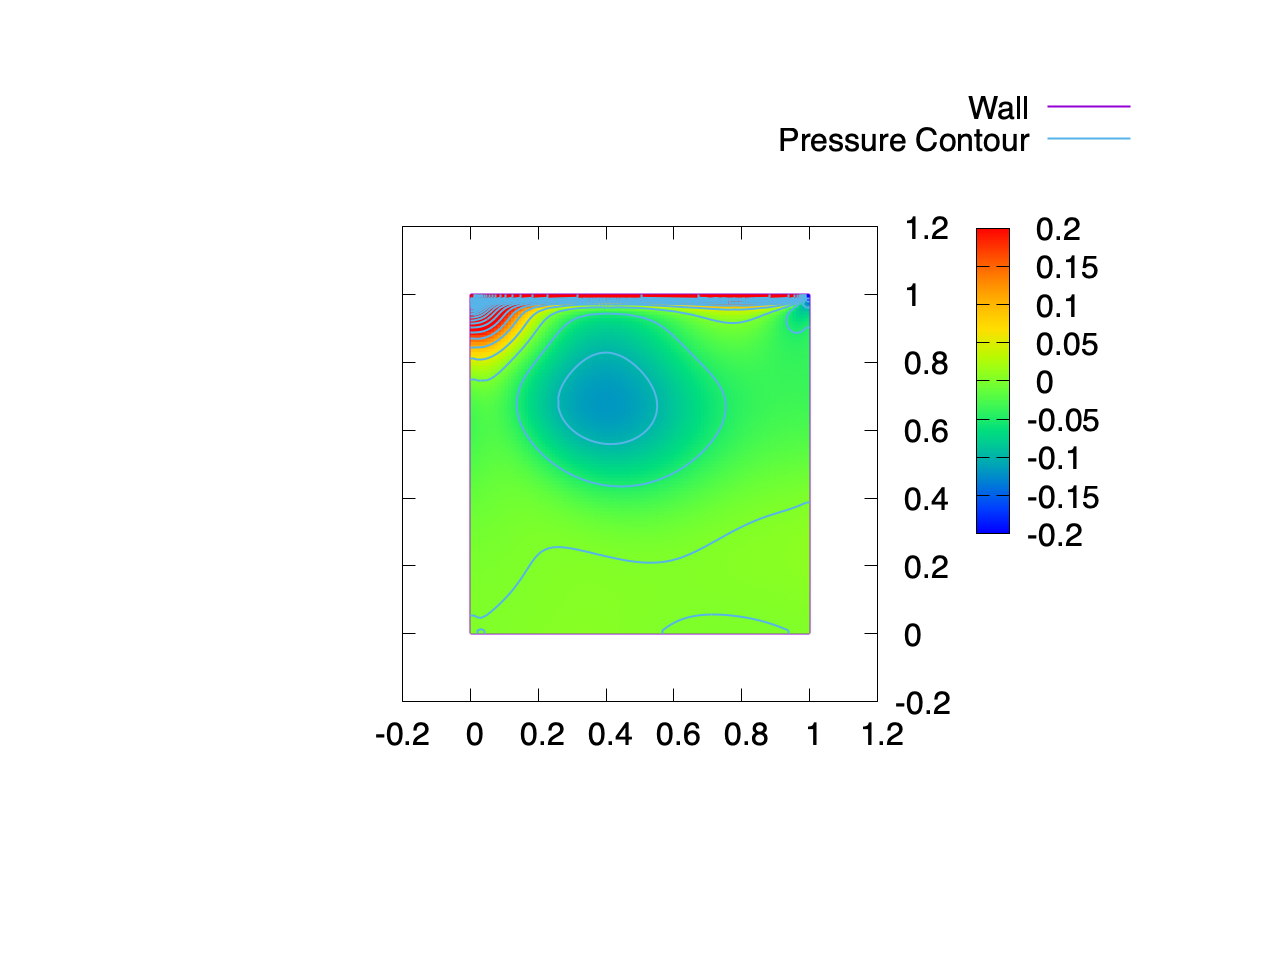
\includegraphics[height=9.5cm]{outputs/img/p_re200.png}
  \caption{等圧線図(ii)}
  \label{fig:p_re200}
\end{figure}
\begin{figure}[H]
  \centering
  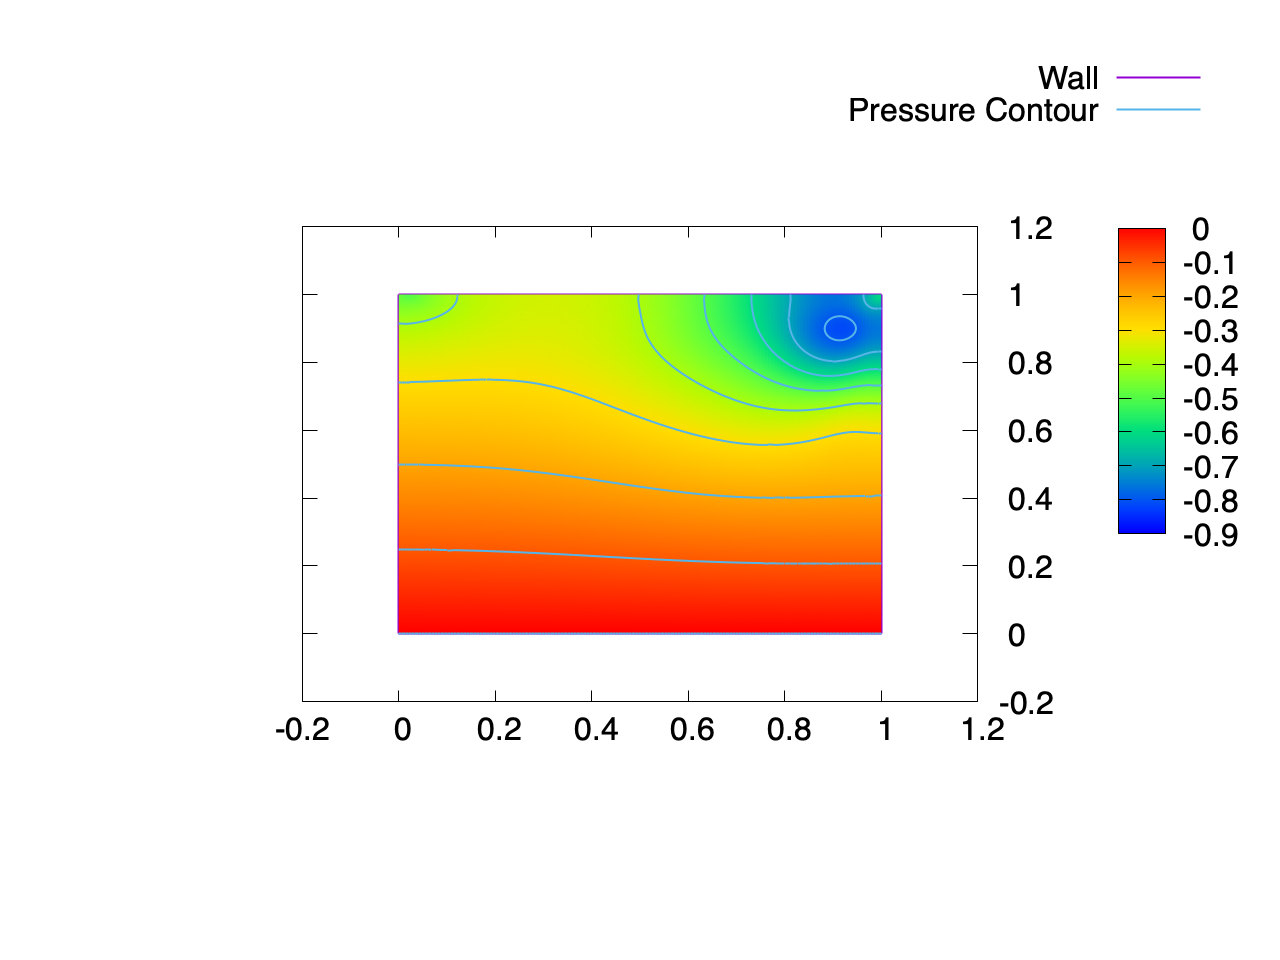
\includegraphics[height=9.5cm]{outputs/img/p_re500.png}
  \caption{等圧線図(iii)}
  \label{fig:p_re500}
\end{figure}

\begin{thebibliography}{9}
  %	\bibitem{1} \url{http://www.hal.t.u-tokyo.ac.jp/lab/ja/index_1.xhtml}
  %    \bibitem{2}Olga Russakovsky*, Jia Deng*, Hao Su, Jonathan Krause, Sanjeev Satheesh, Sean Ma, Zhiheng Huang, Andrej Karpathy, Aditya Khosla, Michael Bernstein, Alexander C. Berg and Li Fei-Fei. (* = equal contribution) ImageNet Large Scale Visual Recognition Challenge. IJCV, 2015.
  \bibitem{1} 研究室資料.流体の数値計算(川口光年先生1976年頃).pdf
  \bibitem{2} 越馬 遼 研究レポート (2021/6/17に提出されたもの)
\end{thebibliography}
\end{document}